\documentclass[a4paper,14pt,titlepage,twoside]{article} 
\usepackage{latexsym} 
\usepackage{textcomp}
\usepackage{mathtext}
\usepackage[T2A]{fontenc} 
\usepackage[utf8]{inputenc} 
\usepackage[russian]{babel} 
\usepackage{indentfirst}
\usepackage[dvips]{graphicx}
\graphicspath{{noiseimages/}}

\title{Аналитическая химия: качественный анализ}
\author{Броннер Илья}
\begin{document}
    \setcounter{page}{0}
    \tableofcontents
    \newpage

    \section{Введение}
        \subsection{Цель}
            Определить состав трёх неизвеснтых веществ (условно названных 01, 10, 11).

        \subsection{Задачи}
            \begin{enumerate}
                \item
                    Найти методы качественного анализа доступные в школьной лаборатории.
                \item 
                    Применить их к нашим веществам
            \end{enumerate}

        \subsection{Методы}
            \begin{enumerate}
                \item
                    Осаждение - получение нерастворимого вещества из нескольких 
                    растворимых.

                    \begin{figure}[h]
                        \center{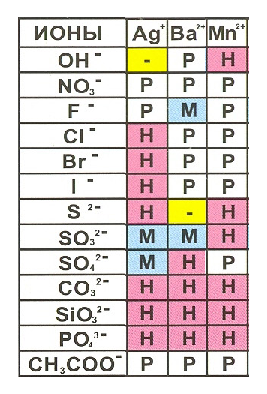
\includegraphics[scale = 0.8]{Table}}
                        \caption{Часть таблицы растворимости использованная при выполнении работы}
                    \end{figure}
            
                \newpage    
                \item
                    Получение газа - получение газа из нескольких твердых или жидких
                    веществ или их комбинаций.

                \item 
                    Окраска пламени - изменение цвета пламени после внесения в него
                    твердого или газообразного вещества.\\

                    \begin{center}
                        \begin{tabular}{ccc}
                            $Sc$ & Темно-красный \\
                            $Li$ & Малиновый\\
                            $Ca$ & Кирпично-красный\\
                            $Na$ & Желтый\\
                            $Mo$ & Желто-Зеленый\\
                            $Ba$ & Желтовато-зеленоватый\\
                            $Cu$ & Ярко-зеленый\\
                            $B$ & Бледно-зеленый\\
                            $Te$ & Зеленый\\
                            $Tl$ & Изумрудный\\
                            $Se$ & Голубой\\
                            $As$ & Бледно-синий\\
                            $In$ & Сине-фиолетовый\\
                            $Cs$ & Розово-фиолетовый\\
                            $Rb$ & Красно-фиолетовый\\
                            $K$ & Фиолетовый\
                        \end{tabular}
                    \end{center}


            \end{enumerate}
        \subsection{Общие сведения о веществах}
            Вещества 01 и 10 хорошо растворимы в воде, оба раствора имеют нейтральную среду
            (по лакмусу и фенолфталеину). Нерастворимые гидроксиды из этих веществ не удалось получить
            добавляя избыток щелочи.

            Вещество 11 растворимо в кипятке (и только в нем) частично, при этом часть
            вещесва нерастворяется независимо от соотношении растворяемого вещества и воды.
            Среда в растворе также нейтральна. Гидрокид полученный добавлением к раствору щелочи нерастворим.

    \newpage
    \section{Определение вещества 01}
        \subsection{Окраска пламени}
            Так как гидрокид полученный из раствора вещества $01$ растворим (см. п. 1.4),
            логично начать его определение с окраски пламени (см. 1.3.3). Так как щелочные
            и щелочно-земляные металы окрашивают пламя, мы сможем легко отличить их от 
            аммония (чей гидроксид также растворим)\\

            Наше вещество не окрасило пламя.\\

            Вывод \newline
            Скорее всего катионом нашего вещества является аммоний.
            Это легко проверить, что и будет сделанно в следующем опыте.
            
        \subsection{Проба на аммоний}
            Проба на аммоний представляет собой перетирание твердого вещества 
            с твердым же гидроксидом натрия (и последующим его нагреванием), с тем чтобы
            почувствовать запах аммиака.\\

            
            Пример

            $NH_4Cl+NaOH_{\mbox{тв.}}\to NH_3\uparrow + H_2O + NaCl$\\

            Наше вещество дало положительную реакцию -
            
            $XY + _aNaOH_{\mbox{тв.}}\to _aNH_3\uparrow + _aH_2O + _aNaY$\\
            
            Вывод\newline
            Наше вещество содержит ион $NH_4{}^+$

        \subsection{Реакция с нитратом серебра}
            Наличие или отсутствие осадка в пробирке с нашим веществом и нитратом серебра
            позволит нам различить анионы $Cl^-, Br^-, I^-,  S^{2-}, SO_3{}^{2-}, PO_4{}^{3-} $ и $ CO_3{}^{2-}$ 
            от $F^-, SO_4{}^{2-}, NO_3{}^-, H_2Po_4{}^2$ и $CH_3COO^-$ соответственно.\\
            
            Пример

            $NaCl + AgNO_3 \to AgCl\downarrow + NaNO_3$
            \par$ Na_2SO_4 + AgNO_3 \ne$\\

            Реакция с нашим веществом прошла без видимых результатов -
            \par$(NH_4)_aX + AgNO_3 \ne$\\


            Вывод

            Анионом нашего вещество может являться один из перечисленных -
            $F^-, SO_4{}^{2-}, NO_3{}^{2-}, H_2PO_4{}^-$ и $CH_3COO^-$.

        \newpage
        \subsection{Реакция с хлоридом бария}
            Наличие или отсутствие осадка поможет нам различать анионы\newline
            $F^-$ и $SO_4{}^{2-}$ от $NO_3{}^{2-}, CH_3COO^-$ и $H_2PO_4{}^-$
            ,соответственно.\\

            Пример
            \par$Na_2NO_3 + BaCl_2 \to BaNO_3\downarrow + 2NaCl$\\

            Реакция с нашим веществом прошла с выделением осадка -

            $(NH_4)_aY + BaCl_2 \to NH_4Cl + BaY\downarrow$\\

            Вывод

            Анионом нашего вещества является один из перечисленных - \newline
            $F^-$ или $SO_4{}^{2-}$.

        \subsection{Реакция с сульфатом магния}
             По реакции с сульфатом магния с нашим веществом можно различить сульфат
             и фторид - фторид магния нерастворим.\\

             Реакция с нашим веществом прошла без видимых результатов - \newline
             $(NH_4)_aY + MgSo_4 \ne$

        \subsection{Результат}
            Согласно результатам предыдущих опытов вещество 01 является сульфатом
            аммония ($(NH_4)_2SO_4$).

            \subsubsection{Реальный вид уравнений}
                $(NH_4)_2SO_4+2NaOH \to 2NH_3\uparrow + Na_2SO_4 + H_2O$
                \par$(NH_4)_2SO_4+AgNO_3 \ne$
                \par$(NH_4)_2SO_4+BaCl_2\to BaSO_4 + 2NH_4Cl$
                \par$(NH_4)_2SO_4+MgSO_4\ne$
            

    \newpage
    \section{Определение вещества 10}
        
        \subsection{Окраска пламени} 
            Наше вещество окрасило пламя в зеленый цвет.\\

            Вывод

            Вещество содержит один из элементов - $Ba, Cu, B, Te$ или $Tl$.

        \subsection{Проба на борные кислоты и их соли}
            Так как зеленую окраску пламени дают несколько элементов, необходимо определить,
            который из них присутствует в нашем веществе. Наиболее вероятными являются
            $Ba, Cu, B$, и различить их можно в ходе одной реакции. Талий же и теллур токсичны
            и скорее всего отсутствуют в школьной лаборатории.\newline

            Проба на борные кислоты (и их соли) проводится путем синтезирования их эфиров,
            и последующего их поджигания. Эфиры борных кислот окрашивают 
            пламя в зеленый цвет.\\

            Пример (в присутствии $H_2SO_4$)
            
            \par $H_3BO_3  + 3C_2H_5OH \to 3H_2O + B(C_2H_5O)_3$\\
            
            \begin{figure}[h]
                \center{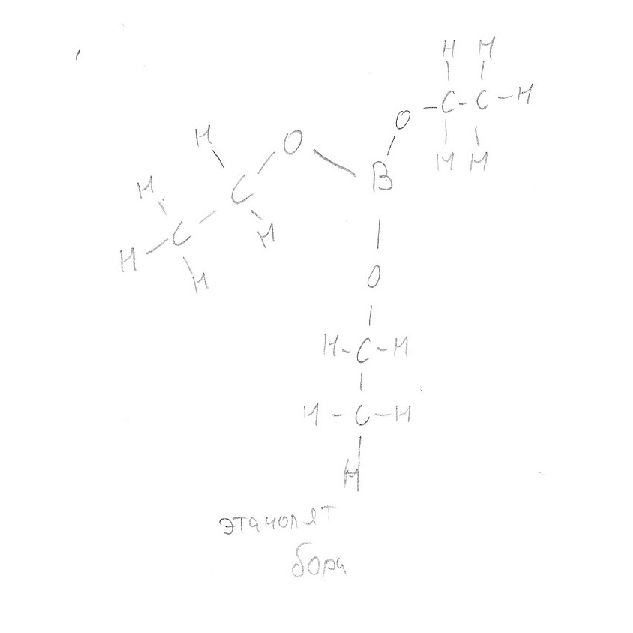
\includegraphics[scale = 0.5]{B(C_2H_5O)_3}}
                \caption{$B(C_2H_5O)_3$}
            \end{figure}

            Наше вещество показало наличие бора\\

            Вывод

            Вещество является солью одной из борных кислот (или самой кислотой) -
            $H_3BO_3$ (ортоборной), $HBO_2$ (мета борной), $H_2B_4O_7$ (тетраборной).\\

            Также можно с уверенностью сказать, что в веществе нет бария - его нерастворимого сульфата
            не было замечено, и не медь - ее сульфат ярко окрашен в синий цвет (чего также не было замечено).

        \subsection{Борные кислоты  и их соли}
            Наиболее распространенными солями борной кислоты являются бура (тетроборат натрия, $Na_2B_4O_7$) и ашарит
            (тетраборат магния,$Mg_2B_4O_4$),\\

            Ашаритом вещество $11$ быть не может, так как гидрокисд магния осаждался бы гидроксидом натрия.
            Бурой же оно не может быть, так как раствор буры давал бы щелочную среду, как соль слабой кислоты и
            сильного основанияю, чего замеченно не было (см. п. 1.4). \\

        \newpage
        \subsection{Различение ортоборной кислоты от тетраборной}
            Так как наше вещество является одной из борных кислот, необходимо как-то их различить.
            Борные кислоты различны по силе - метаборная наиболее слаба, далее "орто-" и "тетра-".
            Так же, они легко переходят друг в друга - \\

            \(H_3BO_3 \stackrel{t^\textdegree}{\to} HBO_2 + H_2O\)
            \par$HBO_2 \stackrel{t^\textdegree}{\to} H_2B_4O_7$\\

            Таким образом, если среда в растворе нашего вещества поменяется на более килую, наше вещество
            является ортобоной кислотой, если нет - тетраборной.\\

            Наше вещество показало не является тетраборной.

        \subsection{Результат}
            Наше вещество является одной из борных кислот $H_3BO_3$ или $HBO_2$.
            \subsubsection{Реальный вид уравнений}  
                $H_3BO_3 + 3C_2H_5OH \to B(C_2H_5O)_3 + 3H_2O$ы
                \begin{figure}[h]
                    \center{\includegraphics[scale = 0.3]{HxByOz+aC_2H_5OH-2}}
                    \caption{$HBO_2+3C_2H_5OH$}
                \end{figure}

                \par$H_2B_4O_7 + 12C_2H_5OH \to 4B(C_2H_5O)_3+ 7H_2O$
                
                 \begin{figure}[h]
                    \center{\includegraphics[scale = 0.2]{HxByOz+aC_2H_5OH-3}}
                    \caption{$H_3BO_3+3C_2H_5OH$}
                \end{figure}
                \newpage
                \par$H_3BO_3 + 3NaHCO_3 \to 3Na_3BO_3 + 3H_2O + 3CO_2\uparrow$
                \par$H_2B_4O_7 + 2NaHCO_3 \to Na_2B_4O_7 + 2CO_2 + 2H_2O$
        \newpage

    \section{Определение вещества 11}
        \subsection{Гидроксид, амфотерность, комплексность}
            Попытка осаждения раствора вещества гидроксидом натрия позволит 
            нам отличать щелочные металлы, водород и аммоний от земляных 
            и щелочно земляных металлов.\\

            Пример
            \par$Al_2SO_4 +NaOH \to 2AlOH + Na_2SO_4$
            \par$KCl + NaOH \ne$\\

            Реакция с нашим веществом прошла с выделением белого осадка.\\

            Вывод 

            Катионом нашего вещества не является щелочной или щелочно землянной
            метал.\\
            
            Далее была проведена проверка гидроксида на амфотерность.
            Амфотерными называют вещества, которые ведут себя одновременно 
            и как основания, и как кислоты.\\

            Пример
            \par$AlCl_3 + 3NaOH \to Al(OH)_3 \downarrow + 3NaCl$
            \par$Al(OH)_3 + NaOH \to Na[Al(OH)_4]$\\

            Аналогично ведут себя гидроксиды большинства d-элементов ($Cr^{+3}, Fe,
            Cu, Zn, Cd$), некоторые s-элементы ($Al, Ga, Pb$) и другие. Также к
            амфотерным гидроксидам можно отнести воду.\\

            Наше вещество явно показало амфотерность, хотя полностью растворено 
            не было.\\

            Наиболее распространенными в школьных лабораториях вещества содержат 
            цинк и алюминий. Их (вернее их гидроксиды) легко различить используя
            25\% раствор аммиака. Гидроксид цинка в нем растворится.\\

            Реакция раствора аммиака с нашим веществом прошла без видимых 
            результатов.\\
    
            Вывод\newline
            Наше вещество не содержит цинка. Скорее всего, катионом 
            нашего вещества является алюминий, но с уверенностью этого сказать нельзя.
            Есть подозрения на комплексную или двойную соль.

        \newpage
        \subsection{Квасцы}
            Квасцы - двойные соли (сульфаты) одновалентного метала с трех валетным.
            Обычно в роли трех валентного метала выступает алюминий, реже хром или железо.\\
                
            \begin{center}
                \begin{tabular}{ccc}
                    $AlNH_4(SO_4)_2 \cdot 12H_2O$ & Алюмоаммонийные квасцы\\
                    $KAl(SO_4)_2 \cdot 12H_2O$ & Алюмокалицные квасцы\\
                    $NaAl(SO_4)_2 \cdot 12H_2O$ & Алюмонатриевые квасцы\\
                    $RbAl(SO_4)_2 \cdot 12H_2O$ & Алюморубидиевые квасцы\\
                    $CsAl(SO_4)_2 \cdot 12H_2O$ & Алюмоцезейные квасцы\\\\
                    $FeNH_4(SO_4)_2 \cdot 12H_2O$ & Жедезоаммонийные квасцы\\
                    $KFe(SO_4)_2 \cdot 12H_2O$ & Железокалийные квасцы\\
                    $KCr(SO_4)_2 \cdot 12H_2O$ & Хромокалицные квасцы\
                \end{tabular}   
                \end{center}

            Из всех выше перечисленных квасцов, нас интересуют только первые,
            так как остальные "алюмо-" {}квасцы гидролизуются по основанию 
            (напомню, среда в растворе вещества нейтральная).\\

            Проверить, является ли наше вещество алюмоаммонийным квасцом, можно
            проведя пробу на аммоний (также как и с первым веществом, см. п. 2.2).\\
            
            Проба на аммоний прошла без видемых результатов.\\

            Вывод\newline
            Наше вещество не является квасцом.



        \subsection{Реакция с нитратом серебра}
            Наличие или отсутствие осадка в пробирке с нашим веществом и нитратом серебра
            позволит нам различить анионы $Cl^-, Br^-, I^-,  S^{2-}, SO_3{}^{2-}, PO_4{}^{3-} $ и $ CO_3{}^{2-}$ 
            от $F^-, SO_4{}^{2-}, HSO_3{}^-, NO_3{}^-, H_2PO_4{}^2$ и $CH_3COO^-$ соответственно.\\
            
            Пример

            $NaCl + AgNO_3 \to AgCl\downarrow + NaNO_3$
            \par$Na_2SO_4 + AgNO_3 \ne$\\

            Реакция с нашим веществом прошла без видимых результатов -
            \par$XY + AgNo_3 \ne$\\


            Вывод

            Анионом нашего вещество может являться один из перечисленных -
            $F^-, SO_4{}^{2-}, NO_3{}^-, H_2PO_4{}^2$ и $CH_3COO^-$.

         \newpage
         \subsection{Реакция с хлоридом бария}
            Наличие или отсутствие осадка поможет нам различать анионы\newline
            $F^-, SO_3{}^{2-}, SO_4{}^{2-}, PO_4{}^{3-}, HPO_4{}^{2-}, CO_3{}^{2-}$ и 
            $SiO_3{}^{2-}$ от $Cl^-, Br^-, I^-, HS^-, \newline 
            HSO_3{}^-, NO_3{}^{2-}, NO_2{}^-, H_2PO_4, 
            HCO_3{}^-$ и $ CH_3COO^-$
            ,соответственно.\\

            Пример
            $Na_2CO_3 + BaCl_2 \to BaCO_3\downarrow + 2NaCl$\\

            Реакция с нашим веществом прошла с выделением осадка.
            $XY + BaCl_2 \to \mbox{Белый осадок}$\\

            Вывод 

            Анионом нашего вещества являются один из перечисленных 
            $F^-, SO_3{}^{2-}, SO_4{}^{2-}, \newline PO_4{}^{3-}, H_2PO_4{}^{2-}, CO_3{}^{2-}$ и 
            $SiO_3{}^{2-}$

        \subsection{Анионы-кандидаты}
            По результатам предыдущих опытов, было установлено, что анионом вещества 
            $11$ могут являться: $F^-$ или $ SO_4{}^{2-}$. $H_2PO_4^{3-}$ мы отвергли в опыте с
            нитратом серебра, так как гидрофосфат серебра разлагается в воде : \\

            $3Ag_2HPO_4 + H_2O \to 2Ag_3PO_4 + H_3PO_4$.\\

            $SiO_3$ был отвергнут после опыта с хлоридом лития - силикат лития нерастворим.
        
\end{document}

